\chapter{相关技术与理论}\label{chap:preliminary}
\markboth{第二章\quad 相关技术与理论}{}
本章将首先给出主题模型的概述,其次对潜在狄利克雷分配模型进行介绍,这是一个经典的用于常规文本分析的主题模型;接着介绍了一个经典的短文本主题模型,狄利克雷多项混合模型;并介绍了这两种模型采用的推断算法吉布斯采样;最后介绍了基于变分自编码器进行推断的主题模型。

\section{主题模型概述}
主题模型通过对文档语料库进行统计分析,能够将包含大量文档的语料库压缩成一个简短的摘要,以揭示语料库中的潜在主题。这个简短的摘要采用主题的形式,即一组相关的词语,因此被称为主题模型。同时,每个文档可以被表示为在这些潜在主题上的一个分布。这种“文档-主题-词”结构提供了语义可解释性,使我们能够更好地理解语料库所包含的主题信息。

图\ref{Chp1_1}\cite{survey_2023}展示了主题模型的一个简单示例,从左到右依次是输入(文档集)、输出(潜在主题)和文本表征(文档-主题分布)。用户输入文档,主题建模算法返回一组与这些文档相关的主题。一些算法会同时返回每个主题中每个单词的权重或相关程度。然后,可以使用这些主题为集合中的文档进行标记,使用户能够了解每个文档和整个集合中主题的重要性。示例文档都是以魔法或中世纪世界为背景的书籍,因此返回的四个主题与这些书中描述的魔法内容相关。主题模型通过识别单词的共现模式并将这些单词模式分组成反映文档内容的主题来分析文本信息。其中一些主题甚至会包含相同的单词(例如示例中的“fairy”)。直观地说,具有一致性、可解释性且重叠单词较少的主题被认为是更高质量的主题。通常情况下,图\ref{Chp1_1}中每个主题所附带的标签都是人为添加的。例如,图中的“Magic”和“Travel”等主题标签通常不会由主题模型分配,一般称为第一个主题、第二个主题等。添加这些主题标签是为了更容易理解文档中已识别的单词集的分布,即主题-词分布。如果一个主题不具有一致性,即包含直观上不应该放在一起的单词,人们往往很难解释这一个主题的含义,那么它们就没办法被赋予适当的标签。

\begin{figure}[!htbp]
    \centering
    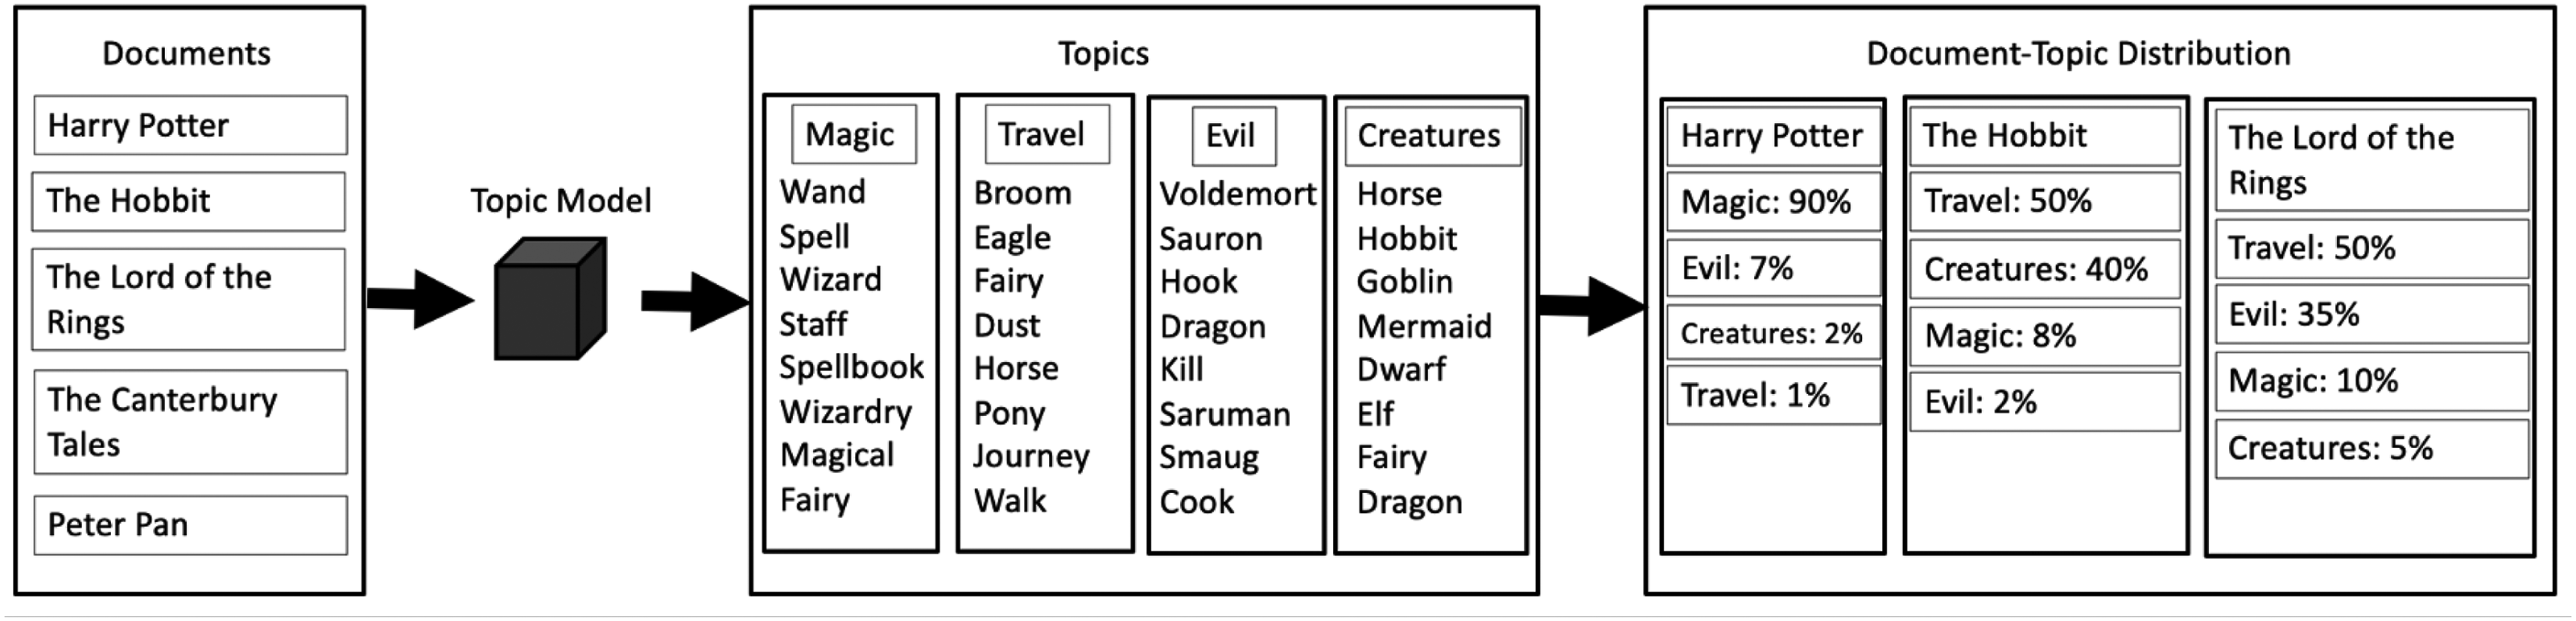
\includegraphics[trim= 0cm 0cm 0cm 0cm, clip=true, width=\textwidth]{chap1/topicModelExample.png}
    \caption{主题模型的示例} 
    \label{Chp1_1}
\end{figure}

\section{经典主题模型算法}
\subsection{潜在狄利克雷分配}
潜在狄利克雷分配(Latent Dirichlet Allocation,LDA)是一种概率主题模型,它可以给出潜在主题对应的词汇概率分布,同时给出文档集中每篇文章对应的主题概率分布。LDA也是一种词袋模型,即不考虑词与词之间的先后关系,一篇文章可以看作是词的集合。一篇文章可以有多个主题,文章中的每个词都对应一个主题。换句话说,LDA模型模拟了一篇文章的生成:先从主题集合中随机地选取一个主题,再以一定的概率从这个主题所对应的词汇集中选取一个词,不断重复上述过程,最终生成一篇文章。表\ref{MathNotationTable}描述了本节主题模型涉及概念所对应的数学符号及其说明。

\begin{table}[ht]
	\caption{在本章涉及概念对应的数学符号以及其说明}
	    \centering
	    \adjustbox{width=0.45\textwidth}{
		\begin{tabular}{cc}
		\toprule
			数学符号 & 说明  \\ 
		 \midrule
			$D$ & 语料库中文本数量  \\
			$V$ & 语料库中词表长度  \\
			$K$ & 主题数  \\ 
			$L$ & 词向量、实体向量的维度  \\   
			$N_{d}$ & 文本$d$包含的单词数  \\ 
			$w_{d,n}$ &  文本$d$中第$n$个单词 \\ 
			$z_{d,n}$ &  文本$d$中第$n$个单词的主题 \\ 
			$\vec{\theta}_{d}$ & 文本$d$对应的主题分布  \\ 
			$\vec{\alpha}$ &   $\vec\theta_{d}$狄利克雷先验超参数\\ 
			$\vec{\beta}_{k}$ & 主题$k$对应的主题-词表分布  \\ 
		   $\vec{\eta}$ &    $\vec\beta_{k}$狄利克雷先验超参数\\ 
		 \bottomrule
		\end{tabular}
		}
	\label{MathNotationTable}
\end{table}

在潜在狄利克雷分配 (LDA) 主题模型中,语料库中的一个文档 $d$ 被表示为,在 $K$ 个主题上具有狄利克雷先验的文档-主题分布 $\vec\theta_d \sim \mbox{Dirichlet}(\vec\alpha)$,而每个主题 $z$ 则通过词汇表上的主题-词分布 $\vec\beta_z\sim \mbox{Dirichlet}(\vec\eta)$ 来建模。其中狄利克雷分布的概率密度函数如公式\ref{Dirichlet}所示,
\begin{equation}
    \label{Dirichlet}
    f(x, x_2, \ldots, x_K; \vec\alpha) = \frac{\Gamma(\sum_{i=1}^K \alpha_i)}{\prod_{i=1}^K \Gamma(\alpha_i)} \prod_{i=1}^K x_i^{\alpha_i - 1}
\end{equation}
狄利克雷分布是一种连续的多变量概率分布,广泛用于概率论和统计学中,特别是作为多项分布的共轭先验分布所使用。因此,如图 \ref{lda} 所示,LDA 的生成过程描述如下:

\begin{enumerate}
    \item[(1)] 对于每一个主题 $k\in {1,\dots,K}$:
    \begin{itemize}
        \item[(a)] 采样一个主题-词分布 $\vec\beta_k\sim \mbox{Dirichlet}(\vec\eta)$ 
    \end{itemize}
	\item[(2)] 对于每一篇文档 $d \in \mathcal{D}$:
	    \begin{enumerate}
		    \item 采样一个文档-主题分布 $\vec\theta_d\sim \mbox{Dirichlet}(\vec\alpha)$
		    \item 对于 $d$ 中的每个单词 $w_{d,n}$:
		        \begin{enumerate}
			            \item 采样一个主题 $z_{d,n} \sim \mbox{Multinomial}(1,\vec\theta_d)$
			            \item 采样一个单词实体 $w_{d,n}\sim \mbox{Multinomial}(1,\vec\beta_{z_{d,n}})$
			        \end{enumerate}
		    \end{enumerate}
\end{enumerate}

\begin{figure}[ht]
    \centering
        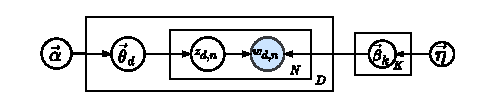
\includegraphics[width=0.8\textwidth]{chap2/LDA.pdf}
        \caption{潜在狄利克雷分配模型(LDA)的概率图模型结构} \label{lda}
\end{figure}

在这个LDA的生成框架下,文档 $d$ 的似然函数是
\begin{equation}
	\label{lda_like}
	p(d|\vec\alpha,\vec\eta)=\int_{\vec\theta_d}\left(\prod_{n=1}^{n_d}\sum_{z_n=1}^k p(z_n|\vec\theta_d)\int_{\vec\beta_k} p(w_n|z_n,\vec\beta_k)p(\vec\beta_k|\vec\eta)\dif\vec\beta_k\right)p(\vec\theta_d|\vec\alpha)\dif\vec\theta_d
\end{equation}

由于在多项式假设下文档-主题分布 $\theta$ 与主题-词分布 $\beta$ 之间的耦合性,LDA 后验推断中的隐变量 $\theta$ 和 $z$ 是难以处理的 \cite{AVITM}。因此主题模型往往采用变分推断\cite{VI}或者吉布斯采样\cite{Gibbs}进行求解。作为MCMC方法中最具有代表性的参数推断方法,吉布斯采样被广泛地应用在主题模型求解过程中。我们会在第\ref{GibbsSampling}节给出更详细的吉布斯采样介绍,这里先给出结果。在 LDA 模型中,先给每篇文章的每个词随机分配一个主题;然后循环遍历每篇文章中的每个词,此时假设当前的词隶属的主题未知,而语料库的文档中剩下的词都已明确其主题,基于此按照吉布斯采样公式计算在该词属于某一个主题的概率,并对当前的词重新采样一个主题,直到语料库的所有文章的词都被重新分配主题,不断重复上述采样过程直到模型收敛。吉布斯采样中的LDA的联合概率分布为
\begin{equation} 
	\begin{aligned}
	p(\mathcal{D},\vec{z} |\vec{\alpha},\vec{\eta}) = 
	\prod_{k=1}^K \frac{\Delta(\vec{n}_{k}+\vec{\eta})}{\Delta(\vec{\eta})}
	\prod_{d=1}^D  \frac{\Delta(\vec{n}_{d}+\vec{\alpha})}{\Delta(\vec{\alpha})}
	\end{aligned}
\label{joinProbLDA2}
\end{equation}


除了当前的单词$w$外,语料库的文档中剩下的词都已明确其主题,基于此按照吉布斯采样公式计算在该词属于某一个主题的概率为
\begin{equation} 
	p(z_w=k |\vec{z}_{\lnot w},\mathcal{D})   
	\propto  \frac{p(\mathcal{D},\vec{z} |\vec{\alpha},\vec{\eta})} 
					{p(\mathcal{D}_{\lnot w},\vec{z}_{\lnot w}|\vec{\alpha},\vec{\eta})} 
	\propto \frac{(n_{k,\lnot w}^v+\eta) }
					{\sum_{v=1}^V (n_{k,\lnot w}^v+\eta)} (n_{d,\lnot w}^k+\alpha)
\label{pzdLDA2}
\end{equation} 
其中$\Delta(\cdot)$是一个函数,例如$\Delta(\vec{\alpha}) = \frac{\prod_{k=1}^K\Gamma(\alpha)}{\Gamma(\sum_{k=1}^K \alpha)}$;$n_{k}$是主题为$k$的单词数,$n_{k}^{w}$是主题$k$下单词$w$出现的次数;$n_{d}^{k}$是文本$d$中属于主题$k$的单词数;$n_{k,\lnot w}^v$为除单词$w$外主题$k$下单词$w$的个数,$n_{d,\lnot w}^k$为除单词$w$外文章$d$属于主题$k$的单词数。

当吉布斯采样完成后,可以求解得到文档-主题分布的参数$\vec\theta$和主题-词分布的参数$\vec\beta$:
\begin{equation} 
	\begin{aligned}
	\beta_{k}^v = \frac{n_{k}^v + \eta}{\sum_{v=1}^V n_{k}^v + V\eta}
	\end{aligned}
\label{phizwLDA}
\end{equation}

\begin{equation} 
	\begin{aligned}
	\theta_{d}^k = \frac{n_{d}^k + \alpha}{\sum_{k=1}^K n_{d}^k + K \alpha}
	\end{aligned}
\label{thetadkLDA}
\end{equation}

\subsection{狄利克雷多项混合模型}
狄利克雷多项混合模型\cite{GSDMM}(Dirichlet Multinomial Mixture Model, DMM)假设数据集是包含多个主题,且每篇短文本只包含一个主题,短文本内的所有单词都由该主题生成。图\ref{DMMProbGraph}为DMM详细的生成过程。

对于整个语料库$\mathcal{D}$,DMM模型的生成式过程描述如下:
\begin{enumerate}
    	
    	\item[(1)] 采样一个语料库-主题分布$\vec{\theta} \sim \mbox{Dirichlet}(\vec{\alpha})$
    	
    	\item[(2)] 对于每一个主题 $k\in {1,\dots,K}$:
    		\begin{enumerate}
    		\item 采样一个主题-词分布 $\vec\beta_k\sim \mbox{Dirichlet}(\vec\eta)$ 
    		\end{enumerate}
    		
    	\item[(3)] 对于每一篇文档 $d \in \mathcal{D}$:
    		\begin{enumerate}
    		\item 采样一个主题$z_{d} \sim \mbox{Multinomial}(\vec{\theta})$
    		\item 对于 $d$ 中的每个单词 $w_{d,n}$:
    			\begin{enumerate}
    			\item 采样一个单词实体 $w_{d,n}\sim \mbox{Multinomial}(1,\vec\beta_{z_{d}})$
    			\end{enumerate}	
    		\end{enumerate}	 
\end{enumerate}
 
\begin{figure}[ht]
	\centering
	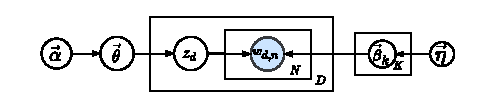
\includegraphics[width=0.8\textwidth]{chap2/DMM.pdf}\\
	\caption{狄利克雷多项混合模型(DMM)概率图模型}\label{DMMProbGraph}
\end{figure}

DMM的隐变量主题-词分布于$\vec{\beta}_{k}$和语料库-主题分布$\vec{\theta}$可以由后验分布$p(\vec{z}|d)$推理得到。同LDA的求解方法,DMM也采用吉布斯采样来求解。当除了短文本$d$外,所有其他文章的主题$\vec{z}_{\lnot d}$和所有文章$\mathcal{D}$已知时,基于吉布斯采样的参数公式如下:

\begin{equation} 
	\begin{aligned}
	p(z_d = k |\vec{z}_{\lnot d},\mathcal{D})   \propto
	\frac{n^{(k)}-1+\alpha}{D-1+K\alpha}
	\frac{\prod_{w \in d} \prod_{j=1}^{n_{d}^w}(n_{k}^w-n_{d}^w+\eta+j-1)} {\prod_{i=1}^{n_{d}}(n_{k}-n_{d}+V\eta+i-1)}
	\end{aligned}
\label{pzdDMM}
\end{equation}
其中 $n^{(k)}$是$D$篇文本中被分配给主题$k$的文章数,$n_{k}$是语料库中被分配给主题$k$的单词数,$n_{(k)}^w$是单词$w$被分配给主题$k$的次数;$n_d$是短文本$d$的长度,$n_d^w$是短文本$d$中单词$w$出现的次数。

当吉布斯采样完成后,可以求解得到文档-主题分布的参数$\vec\theta$和主题-词分布的参数$\vec\beta$:
\begin{equation} 
	\begin{aligned}
	\beta_{k}^w = \frac{n_{k}^w + \eta}{\sum_{w=1}^V n_{k}^w + V\eta}
	\end{aligned}
\label{phizw }
\end{equation}

\begin{equation} 
	\begin{aligned}
	\theta_{k} = \frac{n_{k}+\alpha}{\sum_{i=1}^K n_{i} + K\alpha}
	\end{aligned}
\label{pz-dmm}
\end{equation}

\section{吉布斯采样}\label{GibbsSampling}
上一节中主题模型的推断方法采用了吉布斯采样算法,它是马尔科夫链中随机抽取样本的一种算法。该 算法是循环采样的,同时利用了全条件概率分布来进行采样。每次采样时,只改变其中一个变量,固定其他变量,通过从某个变量相对于其他变量的条件概率分布中进行采样。具体来说,假设我们希望采样的分布由n个变量构成的$p(x_1,x_2,\dots,x_n)$,并且已经为n个变量随机选择了一个初始状态,则吉布斯采样的迭代算法如算法\ref{Gibbs}所示。
\begin{algorithm}[tb]
    \caption{吉布斯采样算法的步骤}
    \label{Gibbs}
    \LinesNumbered
    \KwIn{迭代次数 $I$}
    \KwOut{$(x_1,x_2,\dots,x_n)$的采样结果}
    随机初始化 $(x_1^{(0)},x_2^{(0)},\dots,x_n^{(0)})$\;
    \For{第$i$次迭代, $i\in 1,2,\dots,I$}{
    采样更新$x_1^{(i)}\sim p(x_1|x_2^{(i-1)},x_3^{(i-1)},\dots,x_n^{(i-1)})$\;
	采样更新$x_2^{(i)}\sim p(x_2|x_1^{(i)},x_3^{(i-1)},\dots,x_n^{(i-1)})$\;
	...\\
	采样更新$x_j^{(i)}\sim p(x_j|x_1^{(i)},x_2^{(i)},\dots,x_{j-1}^{(i)},x_{j+1}^{(i-1)},\dots,x_n^{(i-1)})$\;
	...\\
	采样更新$x_n^{(i)}\sim p(x_n|x_1^{(i)},x_2^{(i)},\dots,x_{n-1}^{(i)})$\;
    }
\end{algorithm}

在难以直接进行采样的情况下,吉布斯采样算法是一个很好的选择。该算法的思想是可以从某一个变量 的分布中抽取出一部分样本用于参数估计。上述过程中,从条件概率分布中抽取的样本可以用于近似联合概率分布的样本。

\section{基于变分自编码器的主题模型}
变分自编码器\cite{VAE}(VAE,Variational Autoencoder)是一种深度学习模型,用于无监督学习中的数据生成和编码。VAE 结合了自编码器(Autoencoder)的结构和变分推断(Variational Inference)的理论,主要用于数据的降维和生成任务。在 VAE 中,数据通过编码器映射到一个潜在空间(latent space),这个空间通常是多维高斯分布。编码器的输出不是一个固定的点,而是潜在空间中的分布参数,如均值和方差。然后从这个分布中采样,生成新的数据点,这些点通过解码器映射回原始数据空间。VAE 的关键特性是其损失函数,它包括两部分:一部分是重构误差(如均方误差),用于衡量解码数据与原始数据的相似度;另一部分是KL散度(Kullback-Leibler Divergence),用于衡量编码后的潜在分布与先验分布(通常是标准正态分布)的接近程度。这种结构使 VAE 不仅能够有效地进行数据压缩,还能生成新的、与训练数据类似的样本,应用于图像生成、风格转换等领域。

由于主题模型也可以使用变分推断的方法求解其后验分布的参数,因此一个自然的想法就是将VAE应用于LDA主题模型。如果只考虑文档-主题分布 $\theta$ 而忽略主题分配$z$以及主题-词分布的先验信息,利用符号 $\beta$ 来表示矩阵 $(\vec\beta_1,\vec\beta_2,\dots,\vec\beta_K)^{T}$,将公式\ref{lda_like}中的主题变量$z$进行积分,可以得到
\begin{equation} 
	p(d|\vec\alpha,\vec\eta)=\int_{\vec\theta_d} (\prod_{n=1}^{n_d} p(w_n|\vec\theta_d,\beta))p(\vec\theta_d|\vec\alpha)\dif\vec\theta_d
	\label{lda_like2}
\end{equation}
其中$p(w_n|\theta,\beta)$ 是一个多项式分布,使得LDA模型的生成过程变成:
\begin{enumerate}
	\item[(1)] 对于每一篇文档 $d \in \mathcal{D}$:
	    \begin{enumerate}
		    \item 采样一个文档-主题分布 $\vec\theta_d\sim \mbox{Dirichlet}(\vec\alpha)$
		    \item 对于 $d$ 中的每个单词 $w_{n}$:
		        \begin{enumerate}
			            \item 采样一个单词实体 $w_n\sim \mbox{Multinomial}(1,\vec\theta_d^{T}\beta)$
			        \end{enumerate}
		    \end{enumerate}
	\end{enumerate}
此时文档中的词将独立同分布(i.i.d)地从分布$p(x\vert\vec\theta_d;\beta)=\mbox{Multinomial}(1,\mbox{Softmax}(\vec\theta_d^{T}\beta))$中抽取,被称为“product of experts”\cite{AVITM}。

将 VAE 应用于 LDA 模型时,模型将由一个推断网络(编码器)和一个生成网络(解码器)组成。具体来说,编码器接收文档 $d$ 的词袋(BoW)表示 $x_d$ 作为输入,并输出文档-主题分布 $\theta_d \sim q(\vec\theta_d|x_d;\hat{\vec\alpha})=Dir(\hat{\vec\alpha})$,其中 $q(\vec\theta_d|x_d;\hat{\vec\alpha})$ 是真实后验 $p(\vec\theta_d|x_d)$ 的近似,通常称为变分分布;而$\hat{\vec\alpha} = f_{enc}(x_d)$ 则是通过一个多层感知机(MLP)计算得出。解码器通过给定分布 $p(w_n|\vec\theta_d,\beta)=f_{dec}(\vec\theta_d)$ ,重现接近观测值 $x_d$ 的 $\hat{x_d}$:
\begin{align}
    \hat{\vec\alpha}:&= f_{enc}(x_d;\Pi)\\
    \tilde{\vec\theta_d}&\sim q(\vec\theta_d|x_d;\hat{\vec\alpha})\\
    f_{dec}(\tilde{\vec\theta_d};\beta):&=\mbox{Softmax}(\tilde{\vec\theta_d}^{T}\beta)
\end{align}
在VAE框架下,通过最大化证据下界(ELBO)来优化编码器的参数$\Pi$和解码器的参数$\beta$:
\begin{equation} 
    \mathcal{L}(\Pi,\beta;x_d)=E_{q(\vec\theta_d|x_d)}[\log p(x_d|\vec\theta_d)]-KL(q(\vec\theta_d\vert x_d;\hat{\vec\alpha})\|p(\vec\theta_d;\vec\alpha))
\end{equation}
第一项描绘了文档BoW表示的重构误差,而第二项KL-散度作为一个正则项,使得变分分布接近先验分布。

根据随机梯度变分贝叶斯\cite{},在得到解码器的结果$\hat{\vec\alpha}$之后,需要从 $q(\vec\theta_d|x_d;\hat{\vec\alpha})$ 中采样 $\vec\theta_d$ 来估计在证据下界(ELBO)中的重构误差。通过平均多个样本的贡献来实现,如下式所示:

\begin{equation}
	\mathcal{L}(x_d)=-KL(q(\vec\theta_d|x;\hat{\vec\alpha})||p(\vec\theta_d;\vec\alpha))+\frac{1}{L}\sum_{l=1}^{L}(\log p(x_d|\vec\theta_{d,l},\beta))
	\label{elbo2}
	\end{equation}
其中 L 表示样本的数量。


随机梯度变分贝叶斯的一个基本要求是,隐变量以可微的、非中心化的参数化形式表示,以允许在优化过程中进行梯度计算。然而,狄利克雷分布的形状参数并不满足这一条件。由于狄利克雷分布可以通过伽玛随机变量来模拟,因此拒绝接受采样变分推断 \cite{RSVI} 和伽玛分布的形状增强方法被 DVAE\cite{DVAE}应用于在VAE中对狄利克雷分布进行采样。如果 $z_i \sim \mbox{Gamma}(\alpha_i, 1)$,那么 $\tilde{z}{1:K} = \frac{z{1:K}}{\Sigma_i z_i} \sim \mbox{Dir}(\alpha_{1:K})$。这一点很重要,因为存在一个高效的伽玛分布拒绝采样器:
\begin{equation}
	z=h_\Gamma(\epsilon,\alpha)=(\alpha-\frac{1}{3})(1+\frac{\epsilon}{\sqrt{9\alpha-3}})^3,\,\epsilon\sim \mbox{N}(0,1)
	\label{rejection}
\end{equation}
虽然这个函数由于有些样本会被拒绝而不等同于使用伽玛分布,但对于较高的参数 $\alpha$ 值,往往会有更高的接受率。因此可以应用拒绝采样框架\cite{RSVI}对 $\tilde{z} \sim \mbox{Gamma}(\alpha+B, 1)$ 进行采样,因为 $z \sim \mbox{Gamma}(\alpha, 1)$ 可以表示为 $z = \tilde{z} \prod_{i=1}^B u_i^{\frac{1}{\alpha+i-1}}$,其中 B 是一个正整数,且 $u_i \overset{i.i.d.}\sim \mbox{Uniform[0,1]}$。